\documentclass{beamer}
\mode<presentation>
{
\usetheme{Madrid}
\usecolortheme{seagull}
}

\usepackage{graphicx}
\usepackage{amsmath}
\usepackage{amssymb}

\title[Inheritance]{Inheritance} 

\author{Jaime Canizales} 
\institute[Hunter College] 
{
City University of New York \\ 
\medskip
\textit{jaime.canizales@hunter.cuny.edu} 
}
\date{\today} 
\begin{document}


\begin{frame}
\titlepage 
\end{frame}


\begin{frame} \frametitle{Overview} 
\tableofcontents
\end{frame}


\section{Introduction}
\begin{frame}\frametitle{Introduction}
\begin{block}{Problem Statement}
    What is inheritance ?
\end{block}
\end{frame}


\begin{frame}{Why is this hard?}
\begin{itemize}
\item Why use inheritance ?
\end{itemize}
\end{frame}


\begin{frame}{How inheritance works with constructors}
\begin{itemize} 
\item Pass
\end{itemize}
\end{frame}


\begin{frame}\frametitle{Introduction(cont.)} 
\begin{block}{Solution proposed in paper}
    virtual functions and polymorphism(only works for pointers and references)
\end{block}
\end{frame}    


\begin{frame}{Virtual Functions}
\begin{itemize}
\item Virtual keyword
\item override
\end{itemize}
\end{frame}


\section{Technical Information}
\begin{frame}{Technical Information}
\begin{itemize}
\item why are virtual functions only for runtime
\item Example: For example, you have classes: SuperClass, Subclass1 and Subclass2, and they 
all have a method doACoolThing(). The user presses a button 0, 1 or 2, and,
depending on his input, an instance of the appropriate class is created, and
its doACoolThing() method is called.
\item If you do not choose an inheritance type, C++ defaults to private inheritance (just like members default to private access if you do not specify otherwise).
\end{itemize}  
\end{frame}


\section{Conclusion}
\begin{frame}\frametitle{Conclusion}
\begin{figure}
    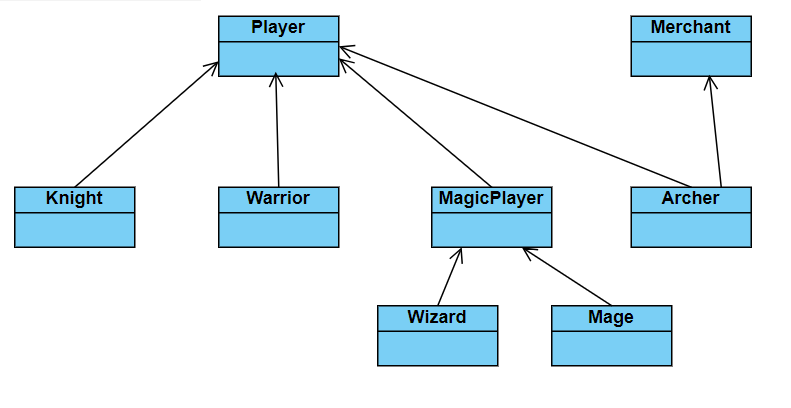
\includegraphics[width=12cm]{code.png}
\end{figure}
\begin{itemize}
\item Software Architecture of code. 
\end{itemize}
\end{frame}


% \begin{frame}
% \frametitle{References}
% \footnotesize{
% \begin{thebibliography}{99} 
% \bibitem[Urain, 2023]{p1} Julen Urain, Niklas Funk, Jan Peters, Georgia Chalvatzaki (2023)
% \newblock SE(3)-DiffusionFields: Learning smooth cost functions for joint grasp and motion optimization through diffusion
% %\newblock \emph{© Springer Science+Business Media, LLC, part of Springer Nature 2020}.
% \end{thebibliography}
% }
% \end{frame}



\end{document}
